\chapter{\IfLanguageName{dutch}{POC: Simulatie}{POC: Simulation}}%
\label{ch:poc}

\section{\IfLanguageName{dutch}{Simulation}{Simulation}}%
\label{sec:sim}%
De \gls{poc} is een simulatie van een 5G-netwerk. Dit wordt opgezet door gebruik te maken van \gls{open5gs}. De \gls{vm} met als \gls{os} Ubuntu, versie 22.04.5 LTS ook wel gekend als Jammy. 

De opbouw van de simulatie zal in 2 fases gebeuren. De eerste is een volledig manuele build. Hier wordt een 5G-netwerk gesimuleerd op een laptop. Dit netwerk bestaat uit een \gls{gnb} en een \gls{ue}. Beiden zullen op eenzelfde toestel in een \gls{vm} worden gerund. De 2de fase is het omzetten van deze manuele build naar een automatische deployment van de \gls{poc}

Als basis hardward configuratie is er gekozen voor een \gls{vm} met 8 Gigabyte RAM en 2 CPU cores. Verder is de netwerkkaart geconfigureerd op het NAT netwerk van VirtualBox zelf.

\section{\IfLanguageName{dutch}{Installatie}{Installation}}%
\label{sec:installation}%

De installatie bestaat uit 3 delen:

\begin{itemize}
    \item Vereiste software
    \item Open5GS
    \item UERANSIM
\end{itemize}

De basis installatie van Open5GS gebeurt volgens de Quickstart van \gls{open5gs}, \textcite{Lee2025a}:

\begin{enumerate}
    \item Installatie van afhankelijkheden/vereisten
    \item Installatie van \gls{open5gs}
    \item Configuratie van \gls{open5gs}
    \item Starten van de \gls{open5gs} services
\end{enumerate}

Nadien wordt \gls{ueransim} geinstalleerd om de simulatie te finaliseren. 

De volledige installatie gids is ook toegevoegd in de bijlagen, zie bijlage \ref{ch:InstallationGuide}.

Er zijn ook eigen configuratie-aanpassingen gebeurt om deze \gls{poc} automatisch te deployen via Vagrant. Hiervoor is er gebruikgemaakt van een Vagrantfile. Deze bevat de hardware configuratie en een link naar het installatiescript voor de simulatie. Echter some configuratie aanpassingen moeten nog steeds manueel worden uitgevoerd.

\begin{lstlisting}[basicstyle=\small, frame=single, breaklines=true, postbreak=\mbox{\textcolor{red}{$\hookrightarrow$}\space}, escapeinside ={\%,}, escapechar={!}, numbers=left, language=sh, caption=Vagrantfile]
Vagrant.configure("2") do |config|
    config.vm.provider "virtualbox" do |vb|
    # Stel de gedeelde map in om automatisch te mounten
    vb.customize ["sharedfolder", "add", :id, "--name", "vagrant_data", "--hostpath", ".", "--automount"]
    end

    config.vm.define "conductor" do |cond|
        cond.vm.box = "gusztavvargadr/ubuntu-server"
        cond.vm.box_version = "2404.0.2503"
        cond.vm.hostname = "Centrale"        # Set the host name of the VM
        cond.vm.network "forwarded_port", guest: 9999, host: 9999, host_ip: "127.0.0.1", id: "open5gs"        # Set portforwarding

        cond.vm.provider "virtualbox" do |vb|        # VirtualBox specific configuration
            # VirtualBox Display Name
            vb.name = "Centrale"
            # VirtualBox Group
            vb.customize ["modifyvm", :id, "--groups", "/BPoc"]
            # 1GB vRAM
            vb.memory = "8192"
            # 1vCPU
            vb.cpus = "2"
        end
        cond.vm.provision "shell", path: "script-cent.sh"
    end
end
\end{lstlisting}

Om deze \gls{vm} te maken wordt er gebruikgemaakt van het commando: \verb|vagrant up|'. Echter door het meermaals testen van de \gls{vm} is er gekozen om een script te schrijven in powershell. Dit script verwijdert de vorige \gls{vm} en start de logging van de terminal. Dit is handig om te detecteren of de \gls{vm} klaar is met de configuratie, maar ook om mogelijk fouten sneller te detecteren.

\begin{lstlisting}[basicstyle=\small, frame=single, breaklines=true, postbreak=\mbox{\textcolor{red}{$\hookrightarrow$}\space}, escapeinside ={\%,}, escapechar={!}, numbers=left, language=sh, caption=Build Script]
Start-Transcript -Path "vagrant.log"
vagrant destroy -f
vagrant up
Stop-Transcript
\end{lstlisting}

\section{\IfLanguageName{dutch}{Configuratie}{Configuration}}%
\label{sec:Config}%

De automatische configuratie wordt gedeployed door het oproepen van een script. Dit is geschreven in bash voor linux, terug te vinden in de bijlagen (hoofdstuk \ref{sec:script}).

Het einde van de automatische configuratie kan worden gedetecteerd aan de hand van de log file ide woerdt gegenereerd tijdens de installatie in de githubrepo. Deze log fie, vagrant.log, is beschikbaar door de shared folder die wordt aangemaakt in het begin van de \gls{vm} installatie. 

Eenmaal de configuratie klaar is moet enkel de handmatige confiuratie gebeuren.

De manuale configuratie bestaat uit 4 delen:

\begin{itemize}
    \item IP check
    \item Open5GS \gls{amf} configuratie
    \item UE configuratie
    \item gNB configuratie
\end{itemize}

Eerst wordt er gekeken naar de huidige IP van de \gls{vm}, dit via het \verb|ip a| commando. Hier kan men het IP adres van de netwerkkaar eth0. Dit IP adres zal worden gebruikt voor verdere configuratie. In het geval van de\gls{poc}, is dit 10.0.2.15

\begin{lstlisting}[basicstyle=\small, frame=single, breaklines=true, postbreak=\mbox{\textcolor{red}{$\hookrightarrow$}\space}, escapeinside ={\%,}, escapechar={!}, numbers=left, language=sh, caption=IP configuratie]
vagrant@Centrale:~/UERANSIM/config$ ip a
1: lo: <LOOPBACK,UP,LOWER_UP> mtu 65536 qdisc noqueue state UNKNOWN group default qlen 1000
    link/loopback 00:00:00:00:00:00 brd 00:00:00:00:00:00
    inet 127.0.0.1/8 scope host lo
        valid_lft forever preferred_lft forever
    inet6 ::1/128 scope host noprefixroute
        valid_lft forever preferred_lft forever
2: eth0: <BROADCAST,MULTICAST,UP,LOWER_UP> mtu 1500 qdisc fq_codel state UP group default qlen 1000
    link/ether 08:00:27:e1:3d:ae brd ff:ff:ff:ff:ff:ff
    altname enp0s3
    inet 10.0.2.15/24 metric 100 brd 10.0.2.255 scope global dynamic eth0
        valid_lft 84941sec preferred_lft 84941sec
    inet6 fe80::a00:27ff:fee1:3dae/64 scope link
        valid_lft forever preferred_lft forever
3: ogstun: <POINTOPOINT,MULTICAST,NOARP,UP,LOWER_UP> mtu 1400 qdisc fq_codel state UP group default qlen 500
    link/none
    inet 10.45.0.1/16 brd 10.45.255.255 scope global ogstun
        valid_lft forever preferred_lft forever
    inet6 2001:db8:cafe::1/48 scope global
        valid_lft forever preferred_lft forever
    inet6 fe80::b792:657a:a404:d020/64 scope link stable-privacy
        valid_lft forever preferred_lft forever
\end{lstlisting}

\subsection{\IfLanguageName{dutch}{Open5GS AMF configuratie}{Open5GS AMF configuration}}%
\label{sec:open5gs_amf}%

Eenmaal het IP adres gekend is worden de hierboven opgelijste configuraties aangepast, beginnend met de \gls{amf}. Hierbij wordt op lijn 23 het ip adres 127.0.0.5 naar het gevonden ip adres 10.0.2.15. Dit is het IP  adres van de ngap server.

\begin{lstlisting}[basicstyle=\small, frame=single, breaklines=true, postbreak=\mbox{\textcolor{red}{$\hookrightarrow$}\space}, escapeinside ={\%,}, escapechar={!}, numbers=left, language=sh, caption=Open5GS amf configuratie]
logger:
    file:
        path: /var/log/open5gs/amf.log
#  level: info   # fatal|error|warn|info(default)|debug|trace

global:
    max:
        ue: 1024  # The number of UE can be increased depending on memory size.
#    peer: 64

amf:
    sbi:
        server:
            - address: 127.0.0.5
            port: 7777
        client:
#      nrf:
#        - uri: http://127.0.0.10:7777
        scp:
            - uri: http://127.0.0.200:7777
    ngap:
        server:
            - address: 10.0.2.15  #CHANGE VALUE
...
\end{lstlisting}

Het is heel belangrijk om de \gls{amf} te herstarten om de nieuwe configuaratie in te laden. Dit wordt gedaan met het commando: 

\subsection{\IfLanguageName{dutch}{gNB configuratie}{gNB configuration}}%
\label{sec:gnb_config}%

\begin{lstlisting}[basicstyle=\small, frame=single, breaklines=true, postbreak=\mbox{\textcolor{red}{$\hookrightarrow$}\space}, escapeinside ={\%,}, escapechar={!}, numbers=left, language=sh, caption=gnb configuratie]
mcc: '999'          # Mobile Country Code value
mnc: '70'           # Mobile Network Code value (2 or 3 digits)

nci: '0x000000010'  # NR Cell Identity (36-bit)
idLength: 32        # NR gNB ID length in bits [22...32]
tac: 1              # Tracking Area Code

linkIp: 10.0.2.15 #CHANGE VALUE   # gNB's local IP address for Radio Link Simulation (Usually same with local IP)
ngapIp: 10.0.2.15 #CHANGE VALUE  # gNB's local IP address for N2 Interface (Usually same with local IP)
gtpIp: 10.0.2.15 #CHANGE VALUE    # gNB's local IP address for N3 Interface (Usually same with local IP)

# List of AMF address information
amfConfigs:
  - address: 10.0.2.15 #CHANGE VALUE
    port: 38412

# List of supported S-NSSAIs by this gNB
slices:
  - sst: 1

# Indicates whether or not SCTP stream number errors should be ignored.
ignoreStreamIds: true
\end{lstlisting}

\subsection{\IfLanguageName{dutch}{UE configuratie}{UE configuration}}%
\label{sec:ue_config}%

\begin{lstlisting}[basicstyle=\small, frame=single, breaklines=true, postbreak=\mbox{\textcolor{red}{$\hookrightarrow$}\space}, escapeinside ={\%,}, escapechar={!}, numbers=left, language=sh, caption=UE configuratie]
# IMSI number of the UE. IMSI = [MCC|MNC|MSISDN] (In total 15 digits)
supi: 'imsi-999700000000001'
# Mobile Country Code value of HPLMN
mcc: '999'
# Mobile Network Code value of HPLMN (2 or 3 digits)
mnc: '70'
# SUCI Protection Scheme : 0 for Null-scheme, 1 for Profile A and 2 for Profile B
protectionScheme: 0
# Home Network Public Key for protecting with SUCI Profile A
homeNetworkPublicKey: '5a8d38864820197c3394b92613b20b91633cbd897119273bf8e4a6f4eec0a650'
# Home Network Public Key ID for protecting with SUCI Profile A
homeNetworkPublicKeyId: 1
# Routing Indicator
routingIndicator: '0000'

# Permanent subscription key
key: '465B5CE8B199B49FAA5F0A2EE238A6BC'
# Operator code (OP or OPC) of the UE
op: 'E8ED289DEBA952E4283B54E88E6183CA'
# This value specifies the OP type and it can be either 'OP' or 'OPC'
opType: 'OPC'
# Authentication Management Field (AMF) value
amf: '8000'
# IMEI number of the device. It is used if no SUPI is provided
imei: '356938035643803'
# IMEISV number of the device. It is used if no SUPI and IMEI is provided
imeiSv: '4370816125816151'

# Network mask used for the UE's TUN interface to define the subnet size
tunNetmask: '255.255.255.0'

# List of gNB IP addresses for Radio Link Simulation
gnbSearchList:
    - 10.0.2.15 #CHANGE VALUE

...
\end{lstlisting}

\subsection{\IfLanguageName{dutch}{Subscriber configuratie}{Subscriber configuration}}%
\label{sec:subscriber_config}%

Voor de configuratie van de subscriber moet er gebruik gemaakt worden van de \gls{open5gs} Web interface. Hiervoor is er een forward-regel zodat deze via de browser van de host-laptop kan worden geraadpleegd op \lstinline!localhost:9999!. Dan wordt de gebruiker verwelkomd met dit aanmeldscherm:

\begin{figure}[H]
    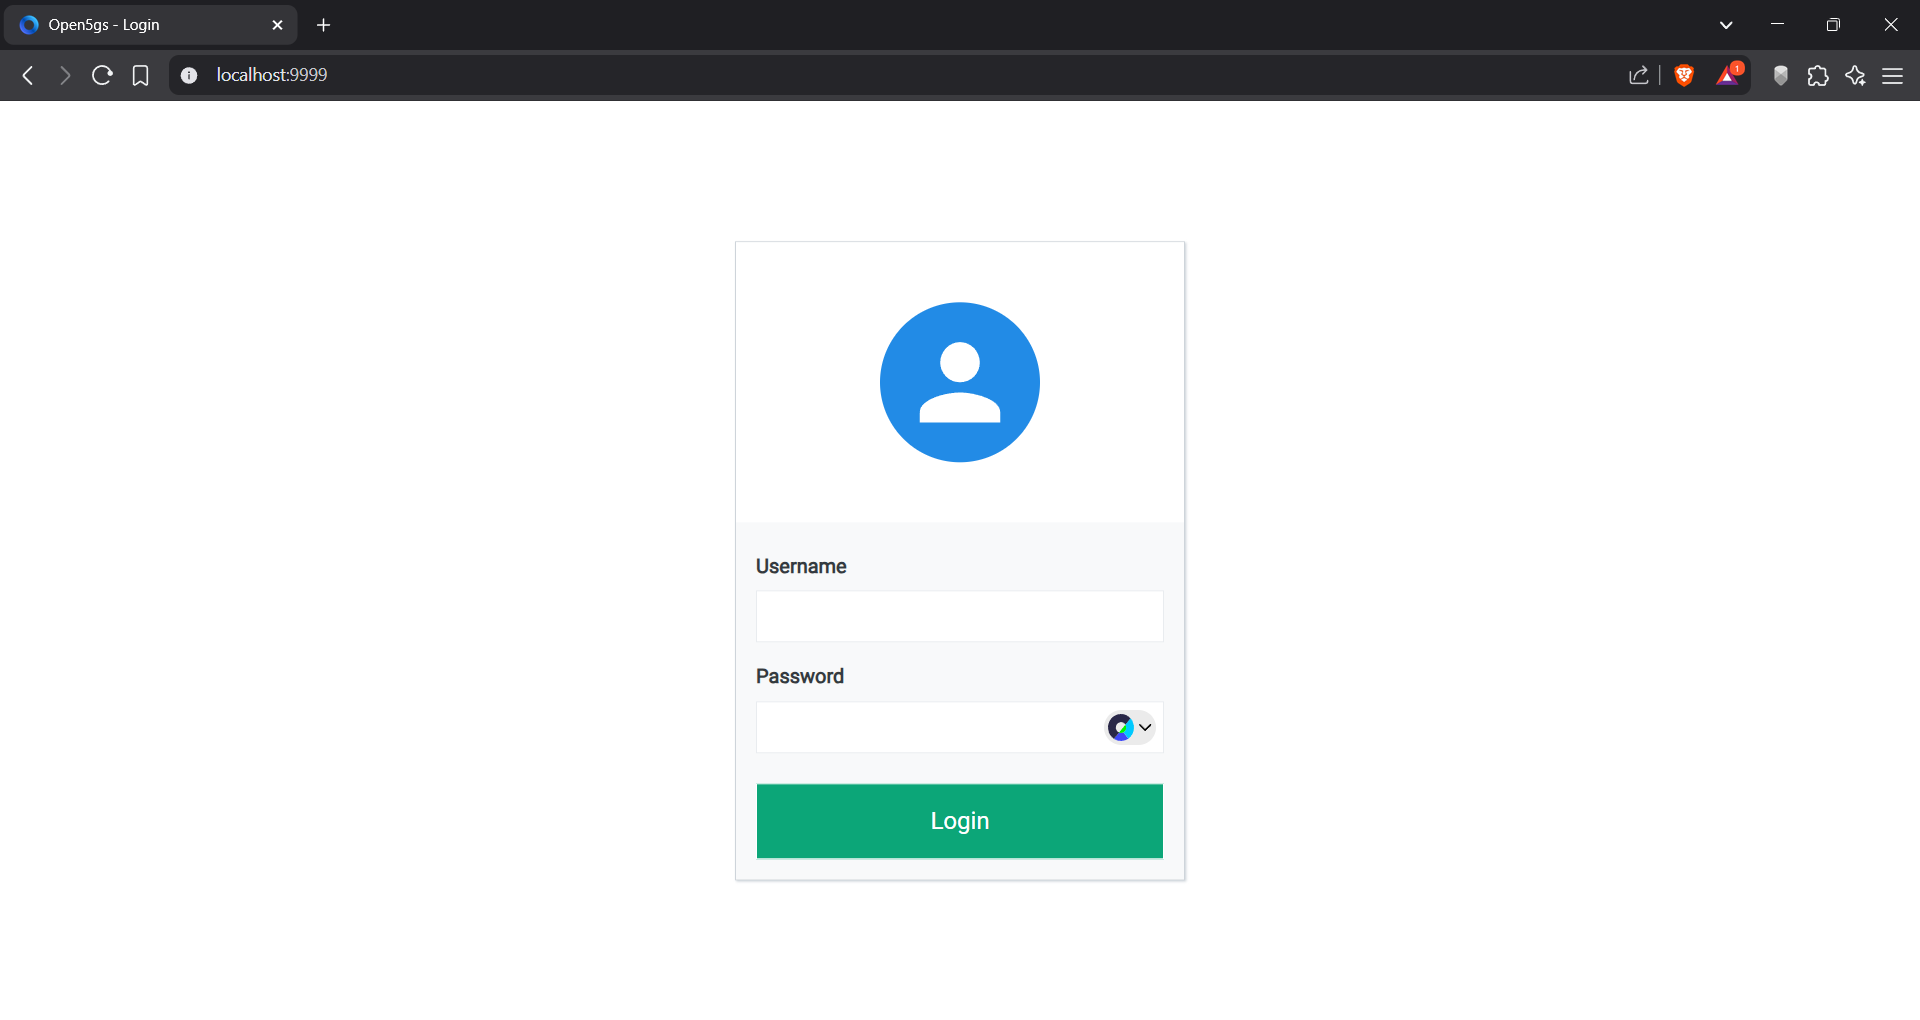
\includegraphics[width=\linewidth]{../graphics/POC-WebUI-Login.png}
    \caption{Aanmeldscherm Open5GS WebUI }
    \label{fig:Aanmeld WebUI}
\end{figure}

Eenmaal aangemeld met de correcte gegevens, terug te vinden in de config-files:

\begin{itemize}
    \item Username: admin
    \item Password: 1423
\end{itemize}

\begin{figure}[H]
    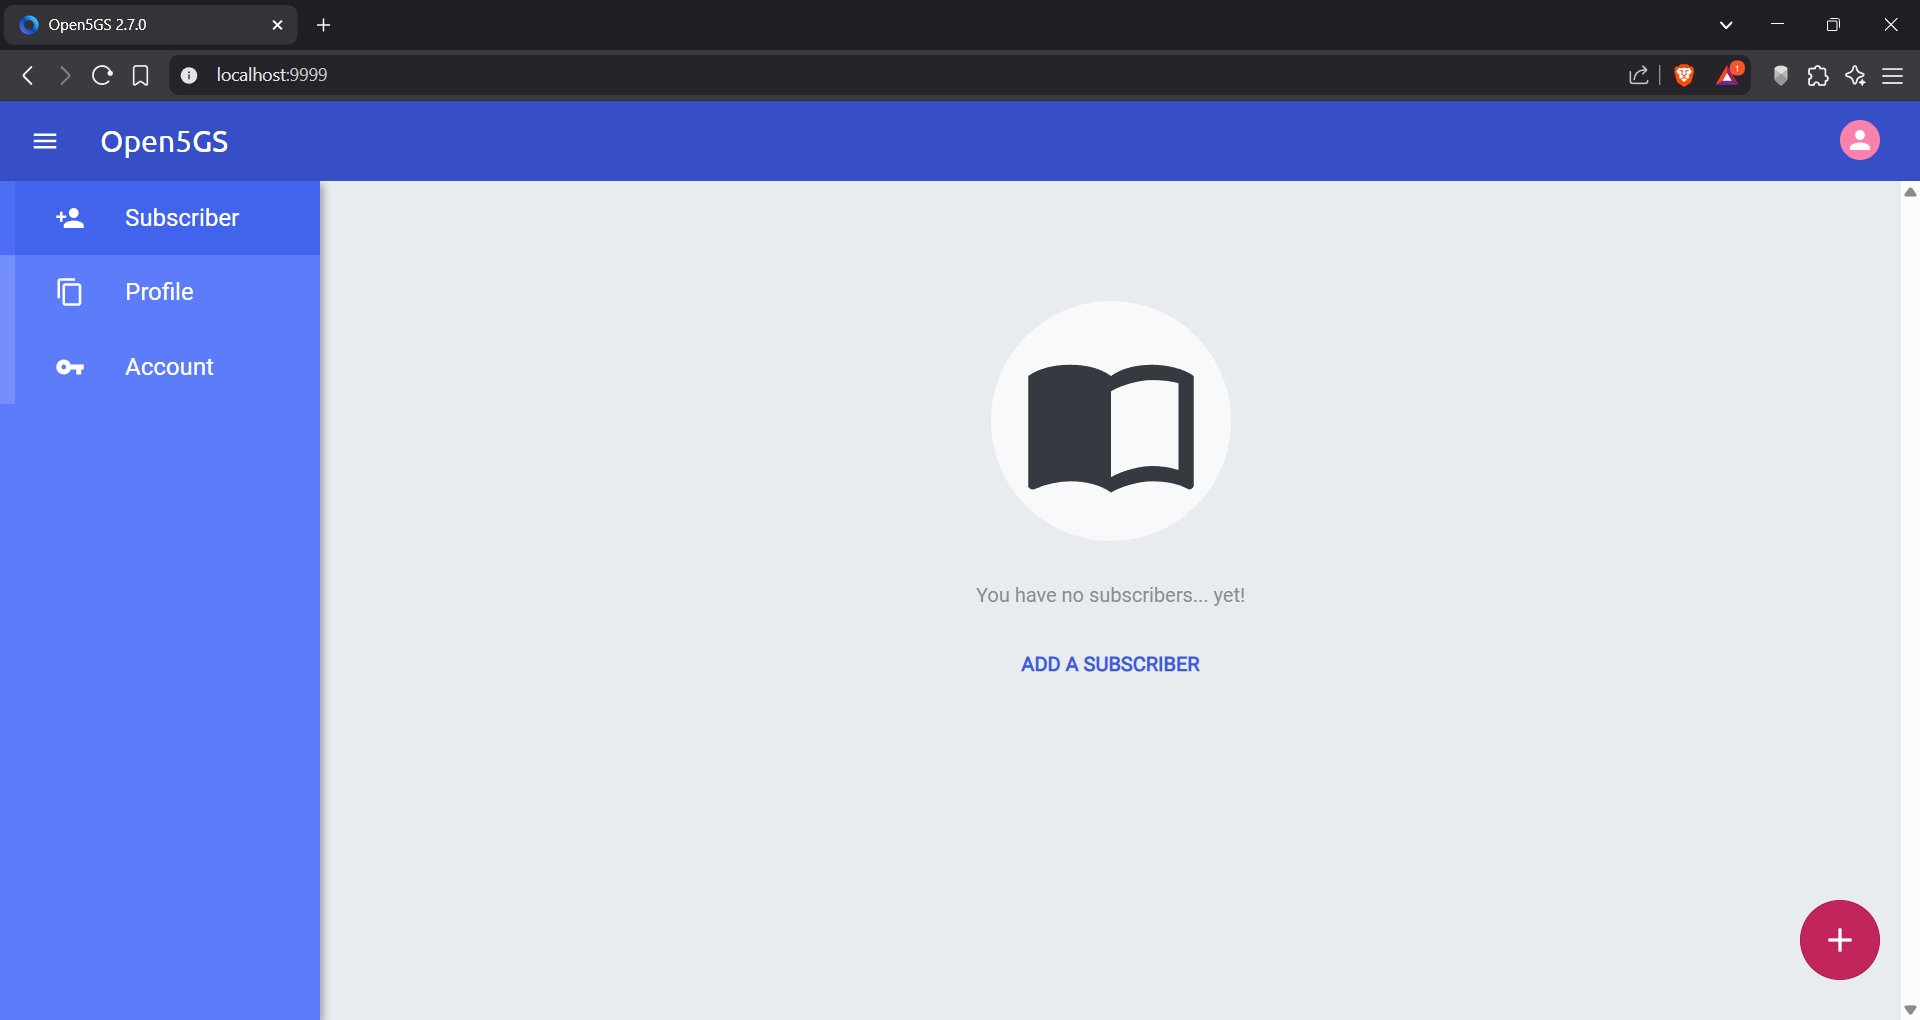
\includegraphics[width=\linewidth]{../graphics/POC-WebUI-home.png}
    \caption{Homescherm Open5GS WebUI }
    \label{fig:Home WebUI}
\end{figure}

Nadien kan een  subscriber worden toegevoegd.
Voor de feitelijke configuratie van de subscriber zijn er gegevens nodig uit de configuaratie file van de \gls{ue}. De gegevens die nodig zijn:

\begin{itemize}
    \item \gls{imsi}
    \item Subscriber Key
    \item \gls{amf}
    \item USIM Type
    \item Operator Key
\end{itemize}

Deze gegevens worden retchstreeks overgenomen uit de configuratie file naar de webinterface voor \gls{open5gs}. Hier kunnen meerdere toestellen als \gls{ue} worden geregistreerd. 
\begin{figure}[H]
    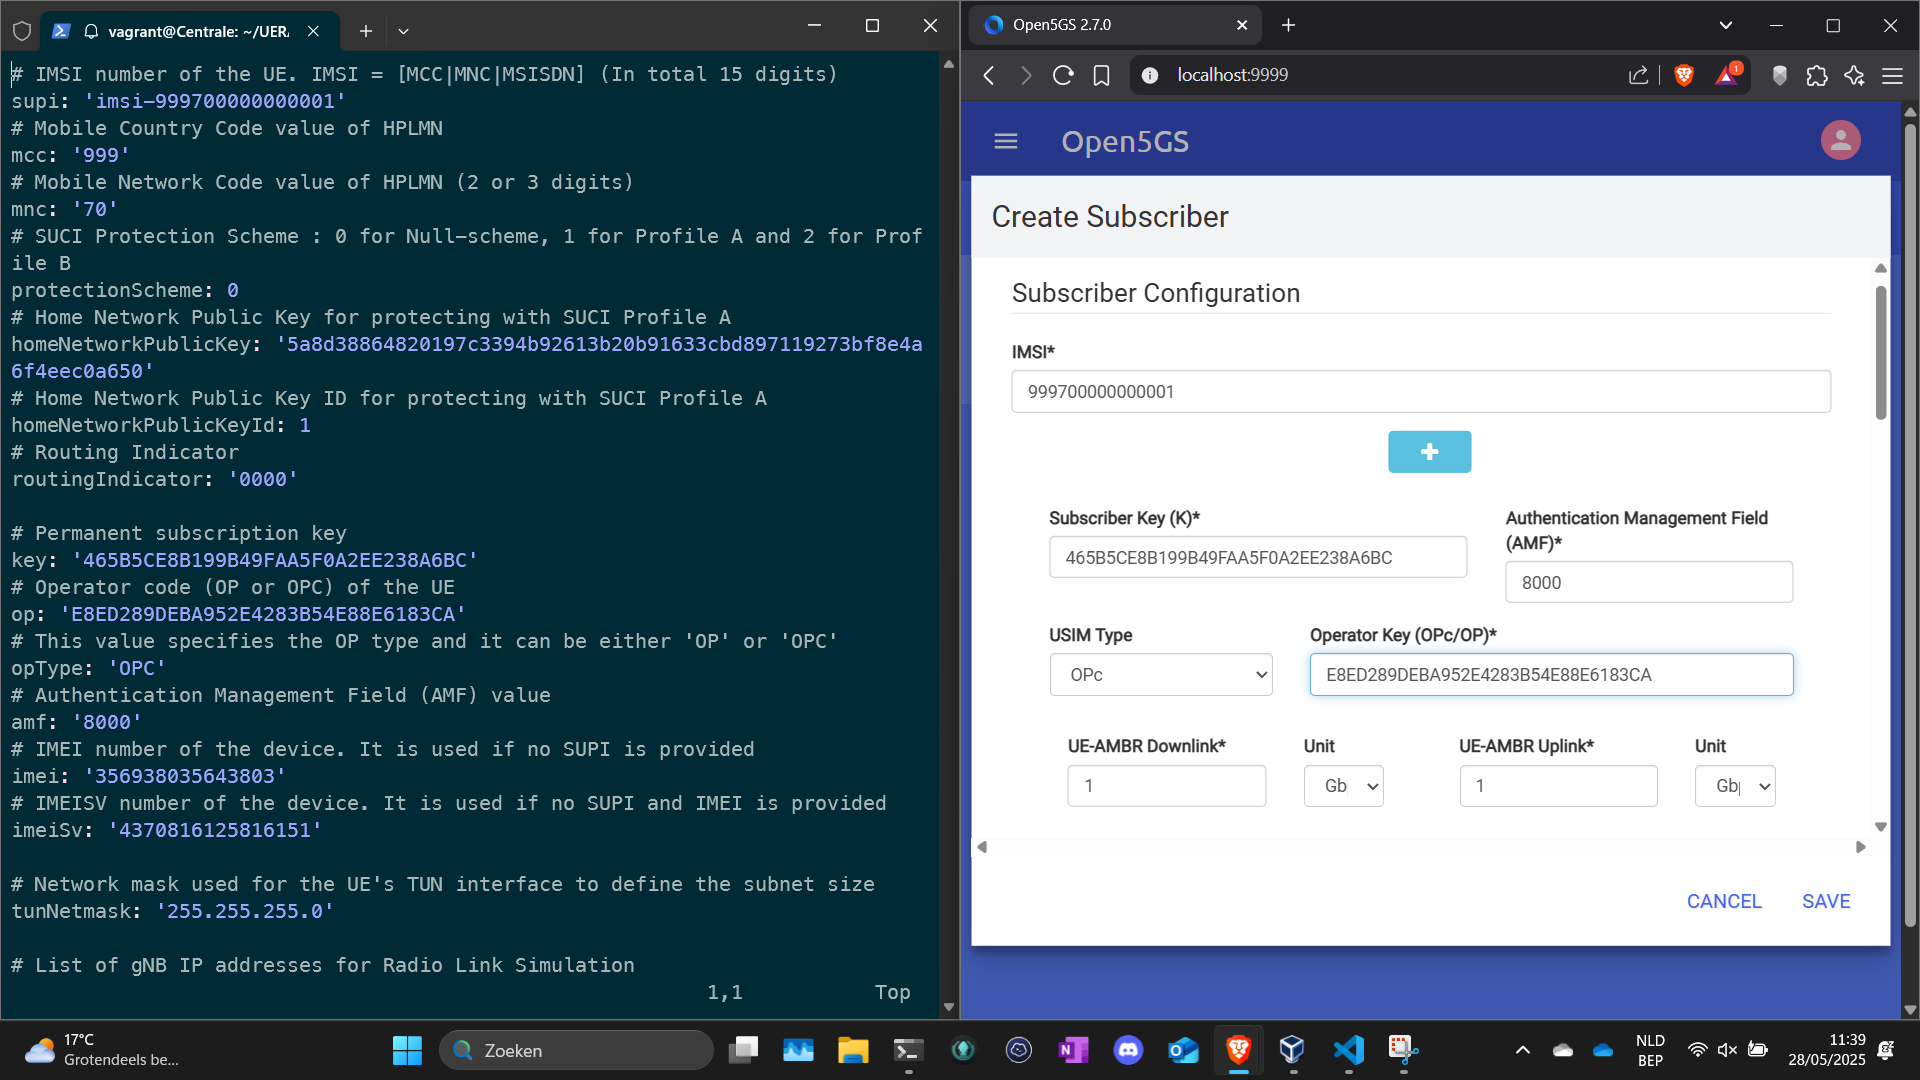
\includegraphics[width=\linewidth]{../graphics/POC-subConfig.png}
    \caption{Configuratie Subscriber}
    \label{fig:SubConfig}
\end{figure}

Na de configuratie sla de subscriber op. Nu is het netwerk volledige geconfigureerd. 

\subsection{\IfLanguageName{dutch}{Run}{Run}}%
\label{sec:run}%

%TODO: Run uitleggen en aantonen dat het werkt ???

\begin{figure}[H]
    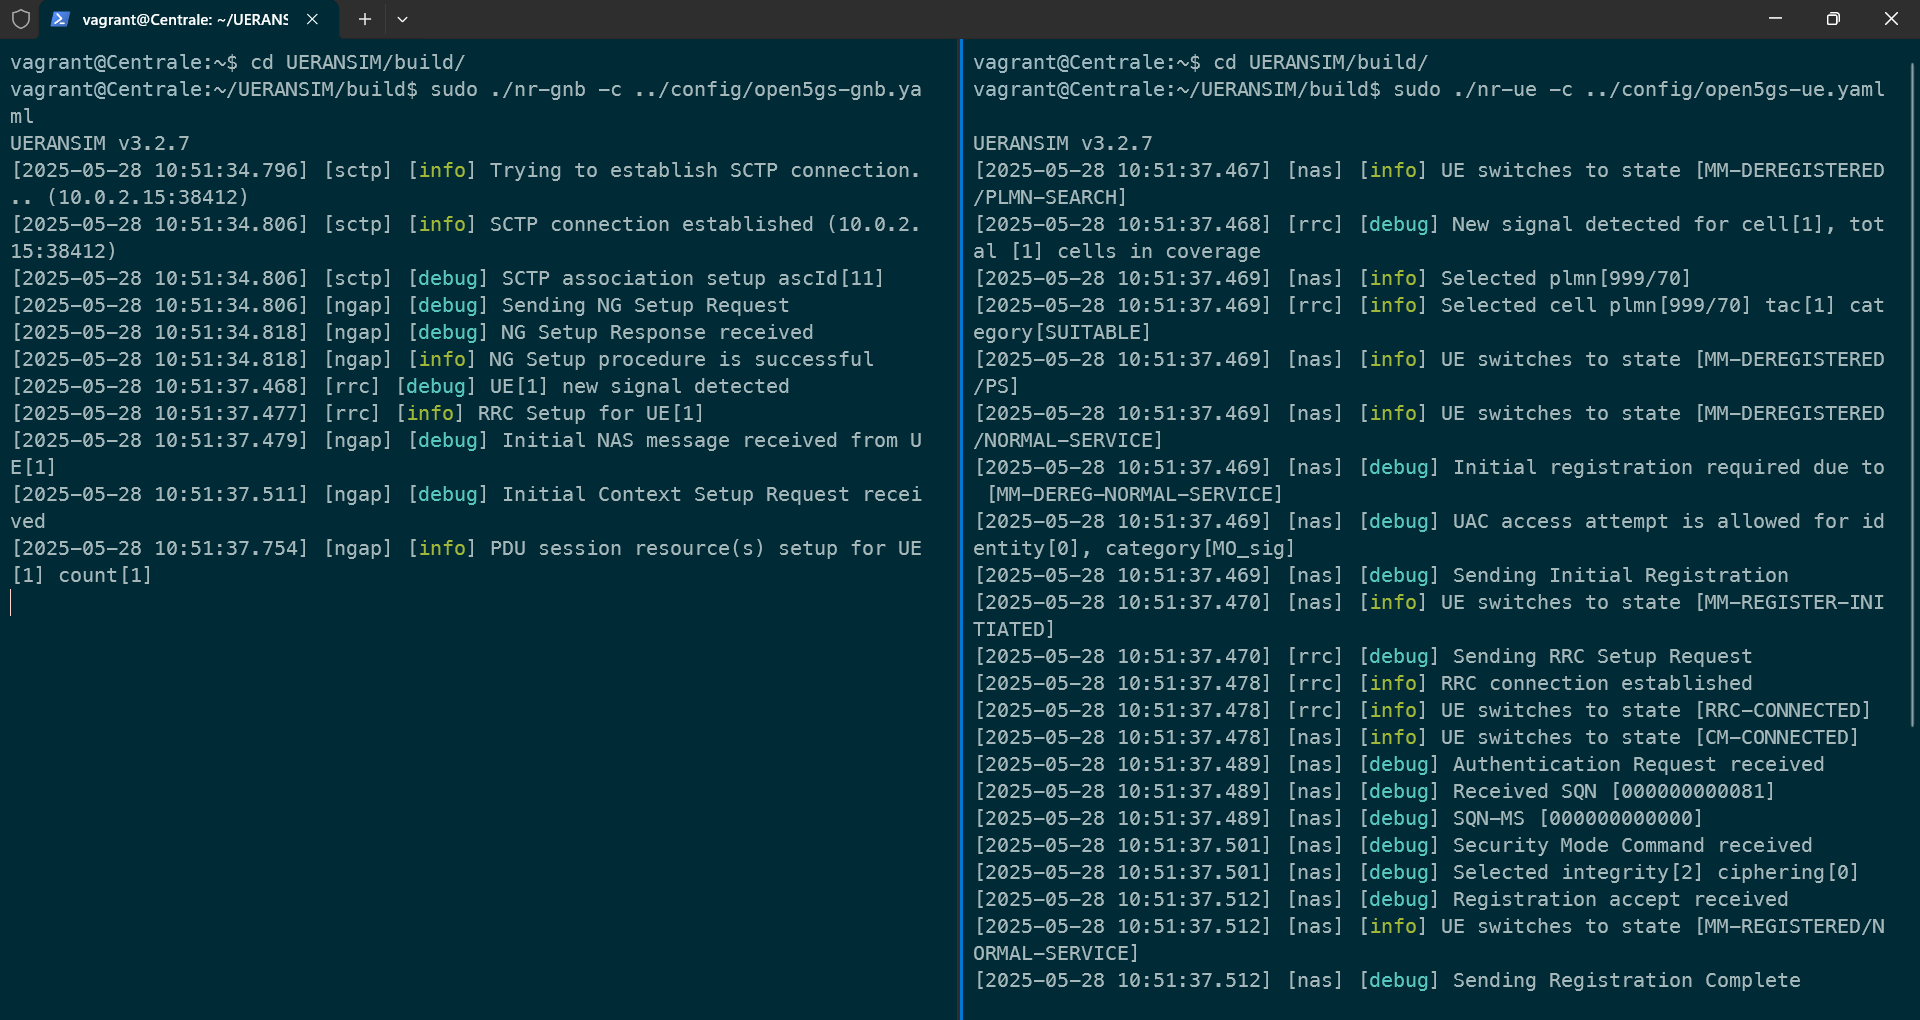
\includegraphics[width=\linewidth]{../graphics/POC-Run-1.png}
    \caption{Running the simulation (Part 1)}
    \label{fig:runPart1}
\end{figure}
\begin{figure}[H]
    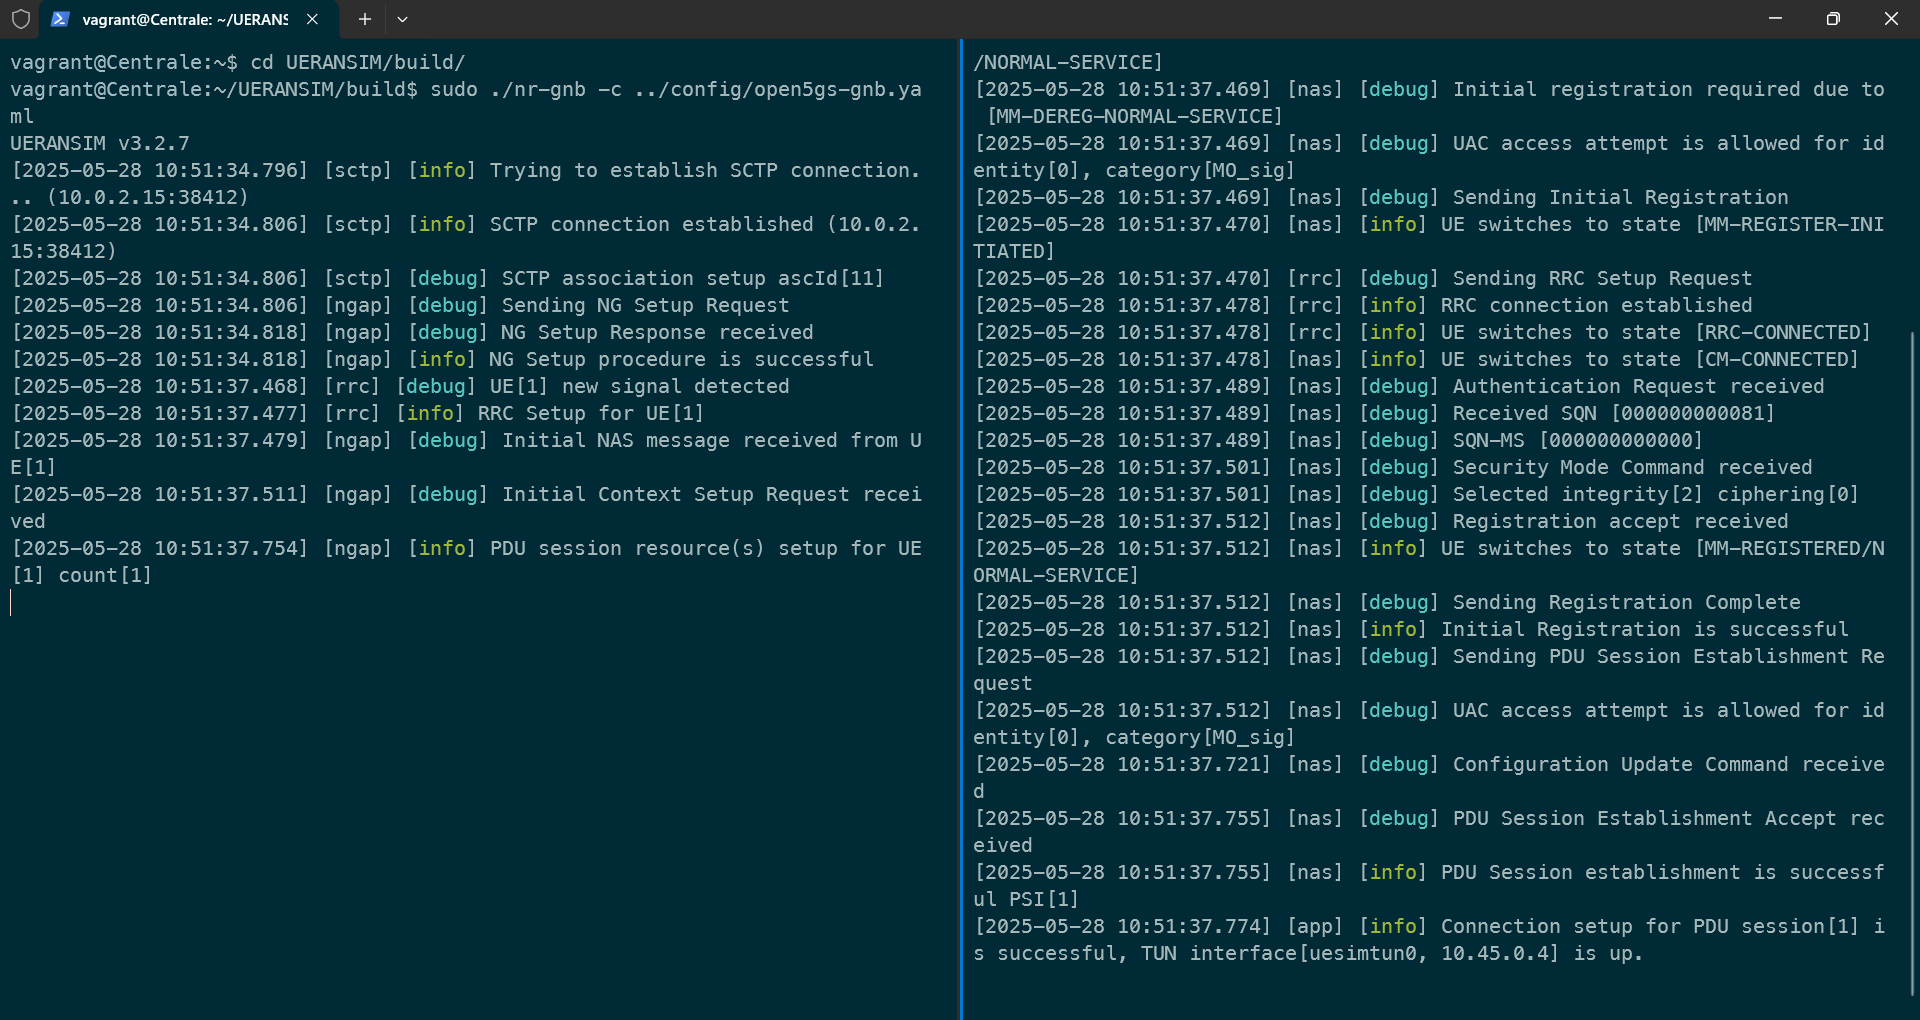
\includegraphics[width=\linewidth]{../graphics/POC-Run-2.png}
    \caption{Running the simulation (Part 2)}
    \label{fig:runPart2}
\end{figure}

\section{\IfLanguageName{dutch}{Andere features}{Additional features}}%
\label{sec:addFeature}%

%TODO: Slicing bespreken

\begin{figure}[H]
    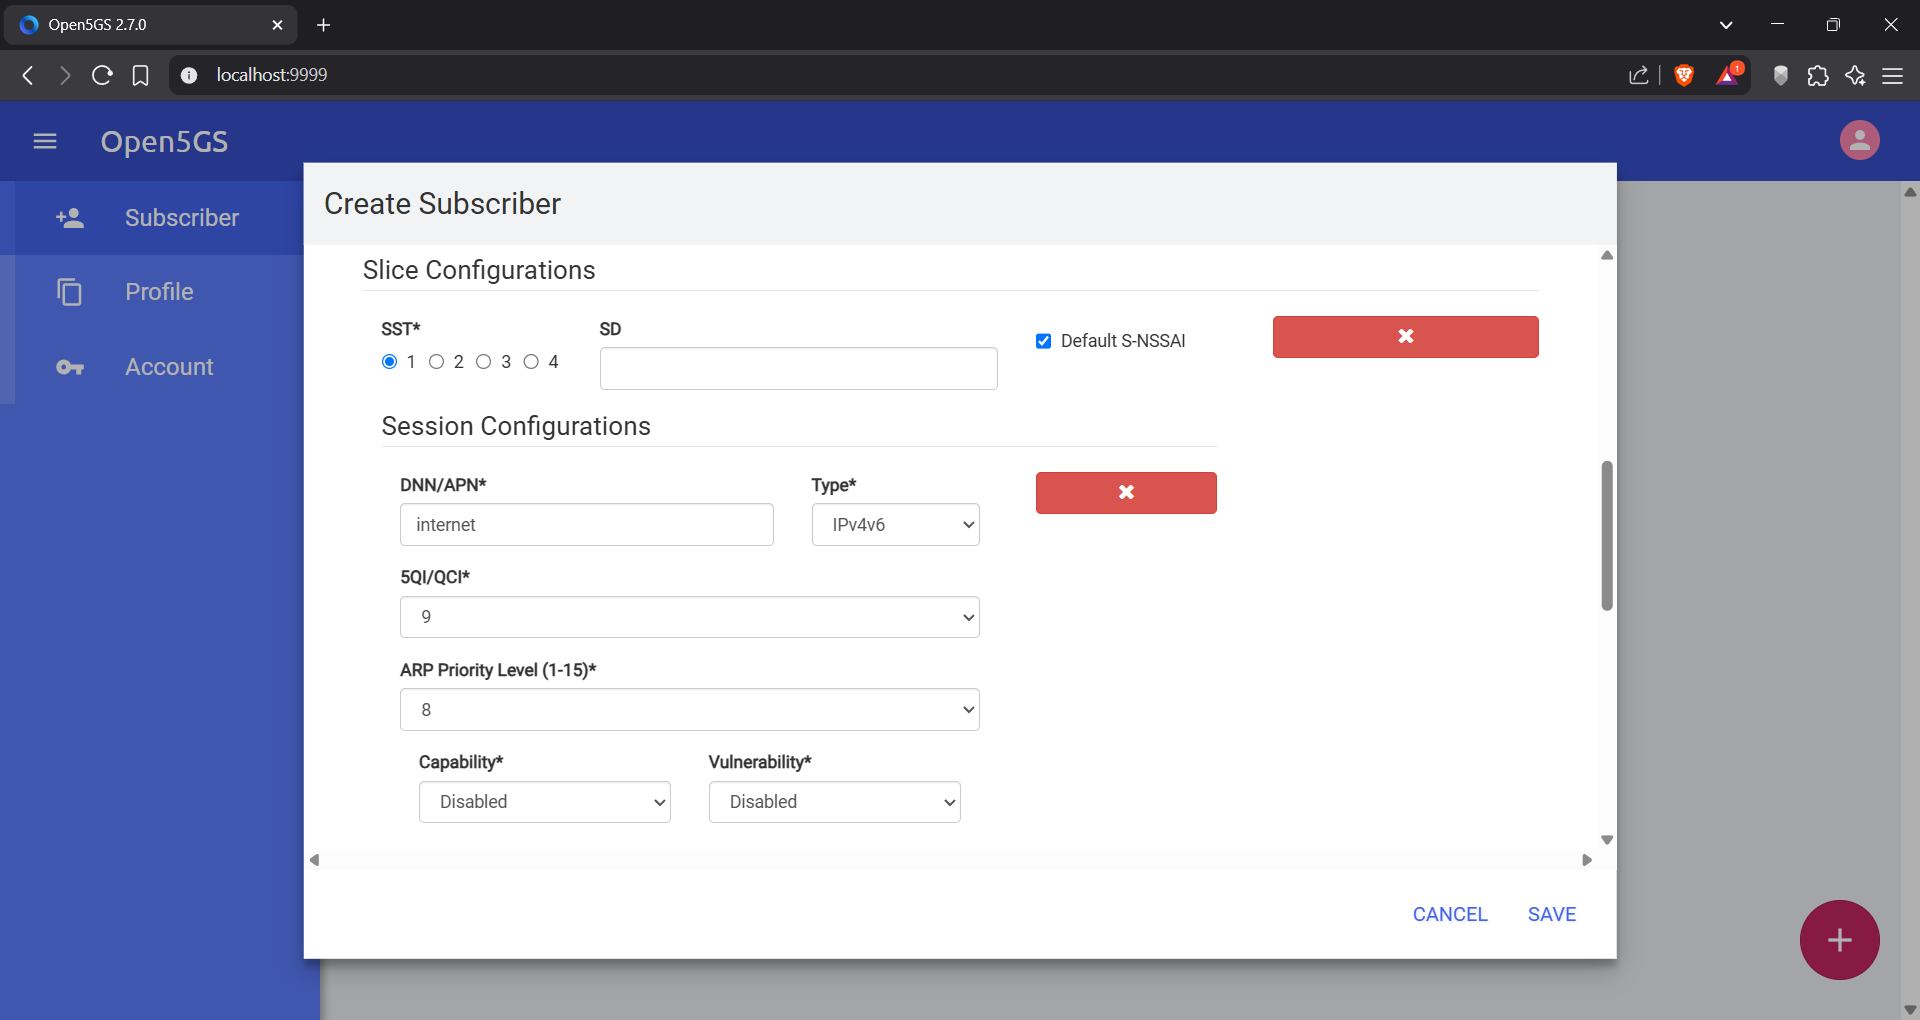
\includegraphics[width=\linewidth]{../graphics/POC-Slicing.png}
    \caption{PoC Slicing}
    \label{fig:pocSlicing}
\end{figure}

\section{\IfLanguageName{dutch}{Mogelijke praktische integraties}{Possible practical integrations}}%
\label{sec:integrations}%

%TODO: Zebra TC27 Handheld Computer en conversie problemen?